\chapter{Introduction to Probability}

\section{Useful Terminologies}

\subsection{Random Experiments}

\begin{definition}[Random Experiment]\index{Random Experiment}
    A process that allows us to gather data or observations. Experiment can be repeated multiple times under the same conditions. The set of possible outcomes of the experiment are known, but the outcome of a specific experiment is not known.
\end{definition}

\begin{example}
    Below are some examples of random experiments. 

    \begin{itemize}
        \item Rolling a die and observing the top-facing number 
        \item Rolling a pair of dice and observing the sum of top-facing numbers 
        \item A patient being administered a painkiller and observing the amount of time in minutes before relief is felt
    \end{itemize}
\end{example}

\begin{definition}[Sample Space]\index{Sample Space}
    The \term{sample space} is the set of all possible outcomes/results from a random experiment, usually denoted by $\Omega$ or $S$. The elements in the sample space are determined by the outcome of interest. Elements and are often denoted by $\omega$.
\end{definition}

\begin{example}
    Below are some examples of the sample space of random experiments. 

    \begin{itemize}
        \item Experiment: Rolling a 20-sided die and observing the top-facing result.

        \begin{itemize}
            \item $\Omega = \{ 1, 2, 3, \dots, 20 \}$ OR 
            \item $S = \{ 1 \le x \le 20, x \in \mathbb{Z} \}$
        \end{itemize}

        \item Experiment: Selecting a random student and observing whether they are a CS student

        \begin{itemize}
            \item $\Omega = \{ \text{CS Student}, \text{Non-CS Student} \}$ OR
            \item $S = \{ 0, 1 \}$ where $\begin{cases} 0 = \text{Non-CS Student} \\ 1 = \text{CS Student} \end{cases}$
        \end{itemize}

        \item Experiment: Select a random student and record the amount of liquids consumed that day 

        $\Omega = \{ L \ge 0, L \in \mathbb{R} \}$
    \end{itemize}
\end{example}

\begin{definition}[Event]\index{Event}\index{Event!Simple Event}\index{Event!Complex Event}
    An \term{event} is a subset of the sample space, usually represented by a capital letter near the beginning of the alphabet. A \term{simple event} has exactly one element of the sample space, while a \term{compound event} consists of multiple elements.
\end{definition}

\begin{definition}[Complement Event]\index{Event!Complement Event}
    The \term{complement event} is the set of outcomes in $\Omega$ that are not in $A$. Can be denoted as one of: $A^c$ (preferred), $\overline{A}$, or $A'$. 
\end{definition}

\begin{example}
    Consider the following example. 

    \begin{itemize}
        \item $A = B^c = \text{roll an even  number} = \{ 2, 4, 6 \}$
        \item $B = A^c = \text{roll an odd number} = \{ 1, 3, 5 \}$
    \end{itemize}

    Here $A$ and $B$ are complement events.
\end{example}

\subsection{Operations on Sets}

\begin{definition}[Union]\index{Union}
    The \term{union} of two events $A$ and $B$ is the set of outcomes that are elements of $A$, $B$, or both. This is denoted as $A \cup B$.

    \begin{itemize}
        \item Union of events is usually described as $A$ \itblue{or} $B$
        \item Note that $A \cup A^c = \Omega$
    \end{itemize}
\end{definition}


\begin{definition}[Intersection]\index{Intersection}
    The \term{intersection} of two events $A$ and $B$ is the set of outcomes that are common to both $A$ and $B$. This is denoted as $A \cap B$, or $AB$ in the textbook.

    \begin{itemize}
        \item Intersection of event is usually described as $A$ \itblue{and} $B$. 
        \item Note that $A \cap A^c = \emptyset$
    \end{itemize}
\end{definition}

\begin{center}
    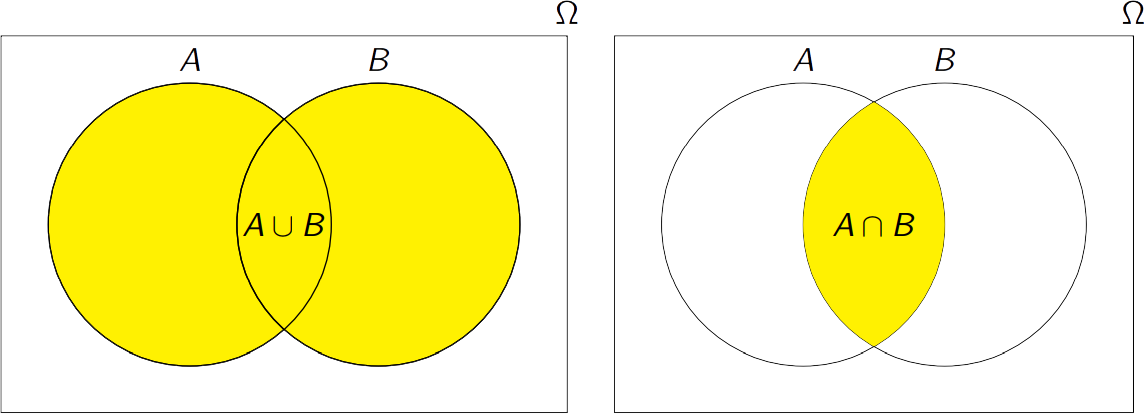
\includegraphics[width=0.75\linewidth]{MultipleEventsVisualized.png}
\end{center}

\begin{example}[Examples of Event Relations]
    Let's keep it simple: suppose we roll two differently coloured\footnote{Note that these two dice are distinguishable, so we would get $\omega = ({\color{red} i}, {\color{lightBlue} j})$} dice and record the paired outcomes. List out the following events:

    \begin{enumerate}[label=\alph*)]
        \item Outcomes are doubles. 

        Let $D$ be the event we roll doubles. 

        $D = \{ ({\color{red} 1}, {\color{lightBlue} 1}), ({\color{red} 2}, {\color{lightBlue} 2}), ({\color{red} 3}, {\color{lightBlue} 3}), ({\color{red} 4}, {\color{lightBlue} 4}), ({\color{red} 5}, {\color{lightBlue} 5}), ({\color{red} 6}, {\color{lightBlue} 6}) \}$

        \item Outcomes sum to $8$. 

        Let $E$ be the event where rolls sum to $8$. 

        $E = \{ ({\color{red} 2}, {\color{lightBlue} 6}), ({\color{red} 3}, {\color{lightBlue} 5}), ({\color{red} 4}, {\color{lightBlue} 4}), ({\color{red} 5}, {\color{lightBlue} 3}), ({\color{red} 6}, {\color{lightBlue} 2}) \}$

        \item Outcomes where one dice has twice the face value as the other. 

        Let $T$ be the event where one die outcome is twice the other. 

        $T = \{ ({\color{red} 1}, {\color{lightBlue} 2}), ({\color{red} 2}, {\color{lightBlue} 4}), ({\color{red} 3}, {\color{lightBlue} 6}), ({\color{red} 6}, {\color{lightBlue} 3}), ({\color{red} 4}, {\color{lightBlue} 2}), ({\color{red} 2}, {\color{lightBlue} 1}) \}$
    \end{enumerate}

    Note that here $E \cap T = \emptyset$ but $E \cup T \neq \Omega$. $E$ and $T$ are \term{disjoint} or \term{mutually exclusive}. $E$ is \bred{not} the complement of $T$. 
\end{example}

subsection{Event Relations}

\begin{definition}[Mutually Exclusive]\index{Mutually Exclusive}\index{Disjoint}
    Two events $A$ and $B$ are \term{mutually exclusive} if the events cannot both occur or occur simultaneously as an outcome of the experiment. This means that the \bred{intersection} of $A$ and $B$ is \bred{empty} and they have no overlapping elements. $A$ and $B$ are also called \term{disjoint} events. 
\end{definition}

In the following Venn Diagram, $A$ and $B$ would be disjoint.

\begin{center}
    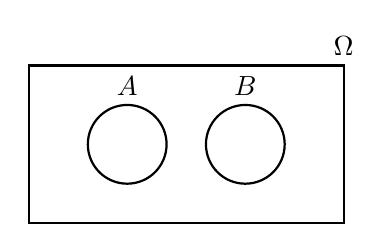
\begin{tikzpicture}
        \node[above] at (2, 1) {$\Omega$};
        \draw[thick] (-2,1) -- (2,1) -- (2,-1) -- (-2,-1) -- cycle;

        \draw[thick] (-0.75,0) circle (0.5);
        \node[above] at (-0.75, 0.5) {$A$};
        \draw[thick] (0.75,0) circle (0.5);
        \node[above] at (0.75, 0.5) {$B$};
    \end{tikzpicture}
\end{center}

\begin{definition}[Independent]\index{Independent}
    Two events $A$ and $B$ are \term{independent} if the occurrence of one event does not alter the probability of occurrence of the other in any way. 
\end{definition}

\begin{example}
    Classify the following paris of events / variables as mutually exclusive, independent, or dependent. 

    \begin{enumerate}[label=\alph*)]
        \item A student surveyed at random: $A = \{ \text{Studies CS} \}$, $B = \{ \text{Studies Stats} \}$

        Dependent. 

        \item A biased coin ($80\%$ Head) is tossed twice: $C = \{ \text{Head on first toss} \}$ and $D = \{ \text{Tail on second toss} \}$

        Independent. 

        \item An individual surveyed at random: $E = \{ \text{Dislikes hiking} \}$ and $F = \{ \text{Likes or indifferent to hiking} \}$

        Mutually Exclusive. 

        \item A playing card is drawn: $G = \{ \text{Card is red} \}$ and $H = \{ \text{Card is Queen of Hearts} \}$

        Dependent. 
    \end{enumerate}
\end{example}

\subsection{Important Laws}

The following laws are useful relationships between unions and intersections of events that can help re-express events in simpler forms.

\begin{theorem}[Commutative Law]\index{Commutative Law}
    $$A \cup B = B \cup A$$
\end{theorem}

\begin{theorem}[Associative Law]\index{Associative Law}
    $$(A \cup B) \cup C = A \cup (B \cup C)$$
    $$(A \cap B) \cap C = A \cap (B \cap C)$$
\end{theorem}

\begin{theorem}[Distributive Law]\index{Distributive Law}
    $$A \cap (B \cup C) = (A \cap B) \cup (A \cap C)$$
\end{theorem}

In addition to the commutative, associative, and distributive laws, \bred{DeMorgan's Laws} present some interesting relationships between union and intersection of events.

\begin{theorem}[DeMorgan's Laws]\index{DeMorgan's Laws}
    For two events $A$ and $B$, 
    $$(A \cup B)^c = A^c \cap B^c$$
    $$(A \cap B)^c = A^c \cup B^c$$
    Or more generally, for the set of events $\{ A_1, A_2, \dots, A_n \}$, 
    $$\left( \bigcup_{i=1}^n A_i \right)^c = \bigcap_{i=1}^n {A_i}^c$$
    $$\left( \bigcap_{i=1}^n A_i \right)^c = \bigcup_{i=1}^n {A_i}^c$$
\end{theorem}

\begin{center}
    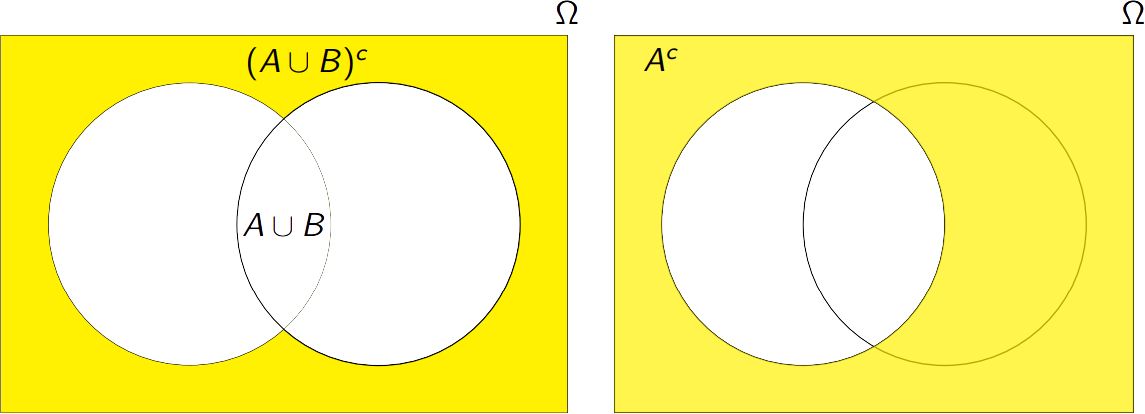
\includegraphics[width=0.75\linewidth]{DeMorgansLawsVisualized1.png}

    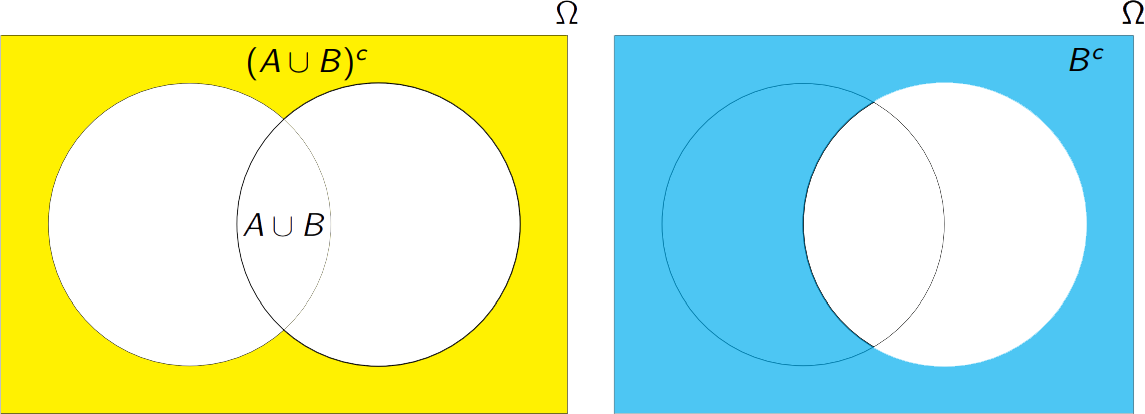
\includegraphics[width=0.75\linewidth]{DeMorgansLawsVisualized2.png}

    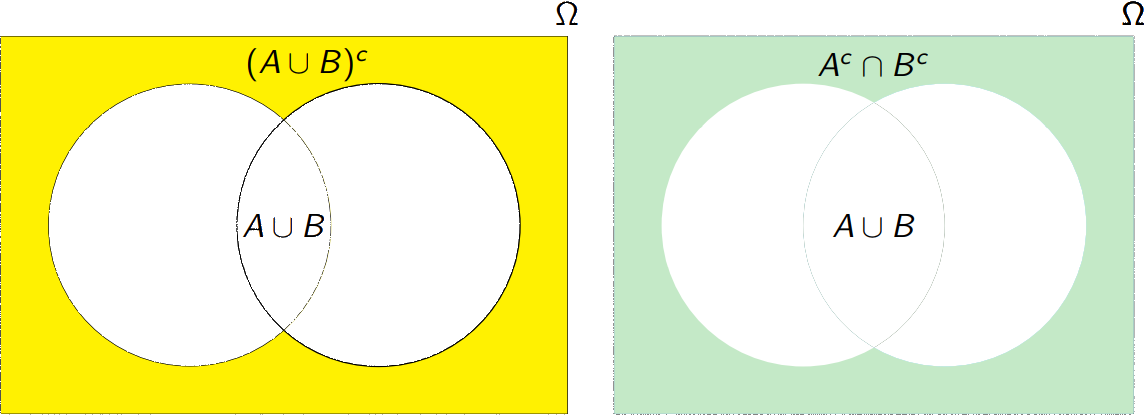
\includegraphics[width=0.75\linewidth]{DeMorgansLawsVisualized3.png}
\end{center}

\section{Probability Functions}

\subsection{Probability Functions}

\begin{definition}[Probability]\index{Probability}
    In a random experiment with sample space $\Omega$, the \term{probability} of an event $A$, denoted as $P(A)$ is a function that assigns to event A a \bred{numerical value} ($P(A) \in [0, 1]$) that measures the chance that event A will occur. 
\end{definition}

There are certain axioms that must hold for probability functions. 

\begin{axiom}[Axiom 1]\index{Axiom 1}
    $$P(A) \ge 0$$
\end{axiom}

\begin{axiom}[Axiom 2]\index{Axiom 2}
    $$P(\Omega) = 1$$
\end{axiom}

\begin{axiom}[Axiom 3]\index{Axiom 3}
    For a set of \bred{disjoint} (mutually exclusive) elements $A_1, A_2, \dots, A_n$ in $\Omega$, 
    $$P \left( \bigcup_{i=1}^n A_i \right) = \sum_{i=1}^n P(A_i)$$
\end{axiom}

Probabilities for outcomes of a random experiment can be represented in many ways. When we have outcomes that can be represented discretely, we can express the associated probability as a function, called a \term{probability function}. A valid probability function must satisfy all the probability axioms.

\begin{definition}[Probability Function]\index{Probability Function}
    Suppose the sample space $\Omega$ can be represented with a finite number of elements: $\Omega = \{ \omega_1, \omega_2, \dots, \omega_n \}$ or a countably infinitely elements $\Omega = \{ \omega_1, \omega_2, \dots \}$, then the \term{probability function} $P$ is a function on $\Omega$ with the following properties:

    \begin{enumerate}
        \item $P(\omega) \ge 0$ for all $\omega \in \Omega$. 
        \item $\sum_{\omega \in \Omega} P(\omega) = 1$
        \item For all events $A \subseteq \Omega$, $P(A) = \sum_{\omega \in A} P(\omega)$
    \end{enumerate}
\end{definition}

\subsection{Probability and Event Relations}

Using the definition of probability, as well as the event relations learned last week, we can relate probabilities of event relations.

\begin{proposition}[Complement Probability]\index{Complement Probability}
    $A \cup A^c = \Omega$ and $A$ is disjoint from $A^c$. Then, $$P(\Omega) = P(A \cup A^c)$$
    We can further derive that $\begin{aligned}[t]
            1      & = P(A \cup A^c) & \text{Axiom 2} \\
            1      & = P(A) + P(A^c) & \text{Axiom 3} \\
            P(A^c) & = 1 - P(A)
        \end{aligned}$
\end{proposition}

\begin{example}
    Suppose we have a box of $20$ dice. Eight of the dice are custom made, and 15 of them are 10-sided dice. Assuming that each die belongs in either of these two categories, can we determine how many are custom made and are 10-sided?

    Let $n(X) =$ number of elements in $X$.

    Let $C =$ custom made die

    Let $T =$ 10-sided die

    We know that $n(\Omega) = 20$, $n(C) = 8$, $n(T) = 15$, and $n((C \cup T)^c) = 0$.
    \begin{align*}
        8 + 15        & = 23                & \text{notice } n(C \cup T) \text{ was counted twice} \\
        \text{excess} & = \text{over count}                                                        \\
        n(C \cap T)   & = 3                                                                        \\
        n(c \cup T)   & = n(\Omega)
    \end{align*}
\end{example}

\begin{example}[Union and Intersection]
    Notice event $B$ (or $A$) can be broken down into the following mutually exclusive events: 
    $$\begin{aligned}[t] B & = (B \cap A) \cup (B \cap A^c) \\ P(B) & = P(A \cap B) + P(A^c \cap B) & \text{Axiom 3} \\ \color{red} P(A^c \cap B) & \color{red} = P(B) - P(A \cap B) \end{aligned}$$

    Note also that $A \cup B$ can also be broken down in a similar way: 
    $$\begin{aligned}[t] P(A \cup B) & = P(A \cup (A \cap B) \cup (B \cap A^c)) \\ & = P(A \cup (B \cap A^c)) & A \cap B \subseteq A \\ & = P(A) + P(A^c \cap B) & \text{Axiom 3, since disjoint} \\ P(A \cup B) & = P(A) + \color{red} P(B) - P(A \cap B) & \text{from above} \end{aligned}$$

    If $A$ and $B$ are disjoint (mutually exclusive), then $P(A \cup B) = P(A) + P(B)$ since $P(A \cap B) = P(\emptyset) = 0$. 
\end{example}

\begin{example}
    In a class of $50$ students, $23$ could not roll their tongue, $15$ had attached earlobes, and $10$ could roll their tongues and had attached earlobes. A student is randomly selected from the class. Let $T$ denote the event that the student can roll their tongue, and $E$ denote the event that they have attached earlobes. Symbolically denote the following events and identify the number of students in each.

    \begin{enumerate}[label=\alph*)]
        \item The student can roll his or her tongue.
        \item  The student can neither roll his or her tongue nor has attached earlobes.
    \end{enumerate}
\end{example}